\section{Creating a custom controler}

%sub\subsection{Introduction}
\begin{frame}
\frametitle{Creating a custom controler}
\framesubtitle{Introduction}
\begin{itemize}
  \item Custom controler for
    \begin{itemize}
  	  \item Integration of own code
  	  \item Customized analysis
  	  \item More complex scenarios which require special modules
    \end{itemize}
  \item Only rewrite the parts you need, but try!
\end{itemize}
\end{frame}

%sub\subsection{First, helpful steps}

\begin{frame}[fragile]
\frametitle{Creating a custom controler}
\framesubtitle{First, helpful steps}
\begin{itemize}
  \item Inherit from \verb|Controler| and add main(String[] args)
  \item Create an instance and call \verb|setOverwriteFiles(true)|
  \item Call the \verb|Controler.run()| method
  \item Open visualizer after \verb|run()| is terminated
  \begin{verbatim}
String[] visargs = {"../output/ITERS/it.0/Snapshot"};
NetVis.main(visargs);\end{verbatim}
\end{itemize}

\end{frame}

%sub\subsection{Handling simulation events}

\begin{frame}[fragile]
\frametitle{Creating a custom controler}
\framesubtitle{Handling simulation events}
\begin{itemize}
  \item Simulation events output of simulation (physical world)
  \item Controler attribute \verb|protected final Events events|
  \item Handler interfaces in \verb|org.matsim.events.handler|
\end{itemize}

\end{frame}

\begin{frame}[fragile]
\frametitle{Creating a custom controler}
\framesubtitle{Handling simulation events}
\begin{itemize}
  \item Write own handler \\
  \begin{verbatim}
MyHandler implements EventhandlerLinkLeave {
  public void handleEvent (EventLinkLeave event) {
    	...do something...
  }
  public void reset(int iteration) {
    	...reset something...
  }
}\end{verbatim}
\end{itemize}

\end{frame}

%sub\subsection{Handling simulation events}

\begin{frame}[fragile]
\frametitle{Creating a custom controler}
\framesubtitle{Handling simulation events}
\begin{itemize}
  \item Create an instance \\
  \begin{verbatim}
  MyHandler handler = new MyHandler();
  \end{verbatim}
  \item Register at Events instance \\
  \begin{verbatim}
  events.addHandler(handler);
  \end{verbatim}
 \end{itemize}
\end{frame}

%sub\subsection{Handling controler events}

\begin{frame}
\frametitle{Creating a custom controler}
\framesubtitle{Handling controler events}
\begin{itemize}
  \item Controler events output of simulation process, e.g.
  \begin{itemize}
  	\item Startup complete
  	\item Begin iteration
  	\item End iteration
  	\item Replanning
  	\item Shutdown
  \end{itemize}
\end{itemize}
\end{frame}


\begin{frame}[fragile]
\frametitle{Creating a custom controler}
\framesubtitle{Handling controler events}
\begin{itemize}
  \item Interfaces in \verb|org.matsim.controler.listener|
  \item Implement and add by \\
  \begin{verbatim}
Controler.addControlerListener(myListenerInstance);
  \end{verbatim}
\end{itemize}

\end{frame}

\begin{frame}[fragile]
\frametitle{Creating a custom controler}
\framesubtitle{Analyse results}
\begin{columns}[T]

\column{7cm}

\begin{itemize}
  \item Controler generates some analysis
  \begin{itemize}
    \item Score statistics
    \item Plans (per 10th iteration)
    \item Snapshots (per 10th iteration)
  	\item Leg histograms (per iteration)
  \end{itemize}
  \item Customized charts via Event handler / listener
  \item Useful tool: \verb|org.matsim.utils.charts|
\end{itemize}

\column{5cm}
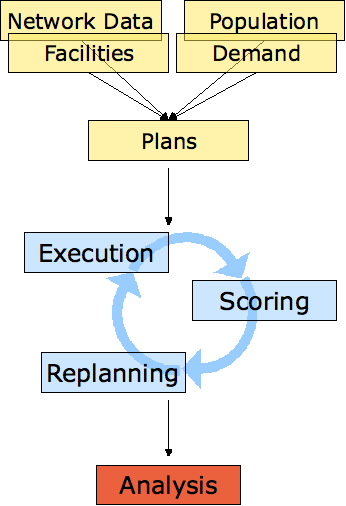
\includegraphics[width=4cm]{../graphics/overviewMatsimAnalysis.png}

\end{columns}
\end{frame}
